\documentclass[../differential_methods.tex]{subfiles}
\begin{document}
\section{Aula 12 - 11 de Maio, 2026}
\subsection{Motivações}
\begin{itemize}
	\item Métodos Multipasso Linear.
\end{itemize}
\subsection{Métodos Multipasso}
\begin{def*}
	Um\textbf{ método multipasso linear de k-passos} é descrito por
	\[
		\sum\limits_{j=0}^{k}\alpha_{j}\mathbf{U}^{n+j} = h \sum\limits_{j=0}^{k}\beta_{j} \mathbf{f}^{n+j},
	\]
	onde \(\mathbf{f}^{n+j}=\mathbf{f}(\mathbf{U}^{n+j}, t_{n+j})\). Adicionalmente, \(\alpha_{k}\neq 0\) e deve-se ter ou \(alpha_{0}\neq 0,\) ou \(beta_{0}\neq 0. \; \square\)
\end{def*}
\begin{figure}[H]
	\begin{center}
		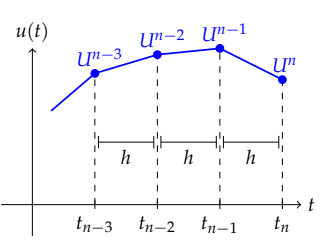
\includegraphics[height=0.6\textheight, width=0.6\textwidth, keepaspectratio]{./Images/multistep_12.png}
	\end{center}
\end{figure}

A dedução da maioria dos métodos baseia-se na integração direta do PVI em qualquer subintervalo entre \(t_{n}\) e \(t_{n+k}\):
\begin{align*}
	 & \mathbf{u}'(t) = \mathbf{f}(\mathbf{u}(t), t)                                                                         \\
	 & \int_{t_{n+r}}^{t_{n+s}}\mathbf{u}'(t) \mathrm{d}t = \int_{t_{n+r}}^{t_{n+s}}\mathbf{f}(\mathbf{u}(t), t) \mathrm{d}t \\
	 & \mathbf{u}(t_{n+s}) - \mathbf{u}(t_{n+r}) = \int_{t_{n+r}}^{t_{n+s}}\mathbf{f}(\mathbf{u}(t), t) \mathrm{d}t.
\end{align*}
Daí, no lado direito, pode-se aplicar uma regra de quadratura.
\begin{example}[Métodos Mutlipassos Linear]
	Alguns métodos multipassos lineares incluem:
	\begin{itemize}
		\item \textbf{Regra do Ponto Médio}: \(\mathbf{U}^{n+2} - \mathbf{U}^{n} = 2h \mathbf{f}^{n+1}\);
		\item \textbf{Método de Simpson}: \(\displaystyle \mathbf{U}^{n+2} - \mathbf{U}^{n} = \frac{h}{3}(\mathbf{f}^{n} + 4 \mathbf{f}^{n+1} + \mathbf{f}^{n+2})\);
		\item \textbf{Adams-Moulton de 2-passos}: \(\displaystyle \mathbf{U}^{n+2} - \mathbf{U}^{n+1} = \frac{h}{12}(-\mathbf{f}^{n} + 8 \mathbf{f}^{n+1} + 5 \mathbf{f}^{n+2})\);
		\item \textbf{Adams-Bashforth de 2-passos}: \(\displaystyle \mathbf{U}^{n+2} - \mathbf{U}^{n+1} = \frac{h}{2}(-\mathbf{f}^{n} + 3 \mathbf{f}^{n+1})\); e
		\item \textbf{Métodos \textit{Backwards Differentiation Formula} (BDF)}: baseiam-se em fórmulas de diferenças finitas regressivas BDF3: \(11 \mathbf{U}^{n+3} -18 \mathbf{U}^{n+2} + 9 \mathbf{U}^{n+1} - 2 \mathbf{U}^{n} = 6h \mathbf{f}^{n+3}\).
	\end{itemize}
\end{example}
\begin{exr}
	Determine as constantes k, \(\alpha_{j}\) e \(\beta_{j}\) para cada um dos métodos acima!
\end{exr}

\begin{tcolorbox}[
		skin=enhanced,
		title=Observação,
		fonttitle=\bfseries,
		colframe=black,
		colbacktitle=cyan!75!white,
		colback=cyan!15,
		colbacklower=black,
		coltitle=black,
		drop fuzzy shadow,
		%drop large lifted shadow
	]
	Note que, quando \(\beta_{k} \neq 0\), a solução \(\mathbf{U}^{n+k}\) depende de \(\mathbf{f}(\mathbf{U}^{n+k}, t_{n+k})\), e consequentemente trata-se de um método implícito! Porém, caso \(\beta_{k}=0\), o método será explícito, pois \(\mathbf{U}^{n+k}\) dependerá apenas de valores calculados previamente.
\end{tcolorbox}

A questão dos diferentes métodos de integração numérica possíveis resulta em diferentes métodos numéricos de resolução do PVI!

\begin{example}[Diferentes métodos de Integração]
	Tomando \(r=0,\; s=1\), a regra de integração numérica do trapézio, encontramos o método do trapézio que discutimos anteriormente.

	Por outro lado, se escolhermos \(r=k-1\) e \(s=k\), junto à regra de quadratura interpolatória em \(t_{n}, t_{n+1}, \dotsc , t_{n+k-1}\) resulta nos \textit{métodos da família Adams-Bashforth.}
\end{example}

Nem tudo são flores: agora, há um problema que não existia no caso dos métodos de passo único -- nem sempre é possível calcular a aproximação \(\mathbf{U}^{1}\) com o mesmo método! Considere o caso do método de Adams-Bashforth de 2 passos:
\[
	\mathbf{U}^{n+2} - \mathbf{U}^{n+1} = \frac{h}{2}(-\mathbf{f}^{n} + 3 \mathbf{f}^{n+1}),
\]
e o primeiro valor possível de se obter uma aproximação com esse método é \(\mathbf{U}^{2} \approx \mathbf{u}(t_{2})\), não sendo possível, portanto, calcular a aproximação \(\mathbf{U}^{1}\) com este método.

Quando isso acontece, o que costuma-se fazer é usar outro método, preferencialmente de passo único, para estimar os valores iniciais \(\mathbf{U}^{0}, \mathbf{U}^{1}, \dotsc , \mathbf{U}^{k-1}\), pois em um método de k-passos, o primeiro valor a ser calculado pelo método é \(\mathbf{U}^{k}\), podendo usar um método de até uma ordem inferior ao erro de truncamento (ordem do método que está utilizando) para não estragar a convergência.

Caso haja convergência, como o número de passos iniciais é sempre fixo e determinado pelo número de passos k do método, devemos necessariamente ter
\[
	\lim_{h\to 0}\mathbf{U}^{\nu }(h) = \underline{\eta }, \quad \nu = 0, 1, \dotsc , k-1,
\]
onde \(\mathbf{u}(0) = \underline{\eta }\) é a condição inicial do PVI.

\begin{def*}
	O \textbf{erro de truncamento de um método multipassos} é calculado com
	\[
		\tau^{n+j} = \frac{1}{h}\sum\limits_{j=0}^{k}\alpha_{j}\mathbf{u}(t_{n+j}) - \sum\limits_{j=0}^{k} \beta_{j}\mathbf{f}(\mathbf{u}(t_{n+j}), t_{n+j}). \; \square
	\]
\end{def*}
Mais ainda, podemos estudar a consistência do Método multipasso linear usando a definição acima:
\begin{align*}
	\tau^{n+j} = & \frac{1}{h}\overbrace{\biggl(\sum\limits_{j=0}^{k}\alpha_{j}\biggr)}^{C_{0}}\mathbf{u}(t_{n}) + \overbrace{\biggl(\sum\limits_{j=0}^{k}(j\alpha_{j}-\beta_{j})\biggr)}^{C_1}\mathbf{u}'(t_{n}) + h \overbrace{\biggl(\sum\limits_{j=0}^{k}\biggl(\frac{1}{2}j^{2}\alpha_{j}-j\beta_{j}\biggr) \biggr)}^{C_2}\mathbf{u}''(t_{n}) \\
	             & +\dotsc + h^{q-1}\underbrace{\biggl(\sum\limits_{j=0}^{k}\biggl(\frac{1}{q!}j^{q}\alpha_{j} - \frac{1}{(q-1)!}j^{q-1}\beta_{j}\biggr)\biggr)}_{C_q} \mathbf{u}^{(q)}(t_{n}) + \dotsc
\end{align*}
Logo, o método será consistente apenas se \(C_{0} = 0\) e \(C_{1}=0\), que equivale a pedir
\[
	\sum\limits_{j=0}^{k}\alpha_{j} = 0 \quad\&\quad \sum\limits_{j=0}^{k}j\alpha_{j} = \sum\limits_{j=0}^{k}\beta_{j}.
\]
\begin{def*}
	Dado um método linear de k passos da forma
	\[
		\sum\limits_{j=0}^{k}\alpha_{j}\mathbf{y}_{n+j} = h \sum\limits_{j=0}^{k}\beta_{j}\mathbf{f}_{n+j},
	\]
	os \textbf{polinômio característicos associados ao método} por
	\[
		\rho(\zeta ) = \sum\limits_{j=0}^{k}\alpha_{j}\zeta^{j} \quad\&\quad \sigma(\zeta ) = \sum\limits_{j=0}^{k}\beta_{j}\zeta^{j}.
	\]
	O polinômio \(\rho(\zeta )\) é chamado \textbf{primeiro polinômio característico}, enquanto que \(\sigma(\zeta )\) é o \textbf{segundo polinômio característico.} \(\square\)
\end{def*}
Os polinômio característicos fazem parte do estudo de consistência, estabilidade e convergência.
\begin{exr}
	Mostre que um MML é consistente se, e somente se, \(\rho(1) = 0\) e \(\rho'(1) = \sigma (1)\);
\end{exr}
\begin{exr}
	Encontre os polinômio característicos dos métodos multipassos exemplificados e avalie a consistência deles.
\end{exr}
Aqui, é importante deixarmos claro o tipo de assunto que vamos estudar:

\begin{def*}
	Um \textbf{estudo de zero-estabilidade} para o problema teste \(u'(t) = 0, \; u(0) =0\), consiste em avaliar o comportamento do método numérico para ele.
	A solução exata do problema é \(u\equiv 0\), e portanto o método numérico também deve recuperar tal solução para ser chamado de zero-estável. \(\square\)
\end{def*}
Em suma, estudar a estabilidade absoluta de um método para PVI consiste em avaliar o comportamento do método em um problema teste de autovalor do tipo \(u'(t) = \lambda u(t)\), com \(\lambda \in \mathbb{C}_{-}\); a definição pode parecer óbvia, mas vamos considerar o seguinte método multipasso linear:
\[
	U^{n+2} - 3U^{n+1} + 2U^{n} = -kf(U^{n}).
\]
Aplicando ao problema teste \(u'(t) = 0\), obtém-se a seguinte fórmula de recorrência:
\[
	U^{n+2} - 3 U^{n+1} + 2U^{n} = 0,
\]
cuja solução é, em termos de valores iniciais \(U^0\) e \(U^{1}\), dada por
\[
	U^{n} = 2U^{0} - U^{1} + 2^{n}(U^{1} - U^{0}).
\]
O que acontece com a solução quando \(U^{0}\neq U^{1}\)? Será que ela se anula? Não! Na verdade, \(U^{n}\rightarrow \infty\).

\begin{def*}
	Um método multipasso linear consistente aplicado à resolução de um problema de valor inicial \(\mathbf{u}'(t) = \mathbf{f}(\mathbf{u}(t), t),\; \mathbf{u}(0) = \underline{\eta },\) é dito \textbf{convergente} se, e somente se, ele for zero-estável. \(\square\)
\end{def*}
Em suma,
\[
	\boxed{\text{Consistência } + \text{ Zero-Estabilidade} \Longleftrightarrow \text{ Convergência}}
\]

Este problema acontece pois o método em questão não satisfaz a propriedade de zero-estabilidade! Assim, determinar a zero-estabilidade de um MML envolve a solução de uma recorrência não trivial, mas ela não é tão prática de ser avaliada puramente pela definição. Para isso, temos um teorema:
\hypertarget{zero_stability}{\begin{theorem*}
		Se as raízes \(\zeta_1, \dotsc , \zeta_{k}\) do polinômio característico \(\rho(\zeta )\) associado a um MML de k-passos satisfazem as seguintes condições:
		\begin{align*}
			 & | \zeta_{j} |\leq 1 \quad \forall j=1, 2, \dotsc , k;
			 & | \zeta_{j} | < 1 \text{ sempre que }\zeta_{j} \text{ for \hyperlink{multiple_root}{\textit{raiz múltipla}}}.
		\end{align*}
		Então, o MML é zero-estável.
	\end{theorem*}}

\begin{exr}
	Mostre que métodos multipasso lineares com \(k=1\) são sempre zero-estáveis, e portanto, sempre convergentes.
\end{exr}

Note que, mesmo sendo zero-estável, um método ainda pode sofrer dos mesmos problemas de estabilidade absoluta já estudados anteriormente. Considere o problema \(u'(t) = \lambda u(t),\; u(0) = \eta \), discretizando-o por um MML:
\[
	\sum\limits_{j=0}^{k}\alpha_{j} U^{n+j} = h \sum\limits_{j=0}^{k}\beta_{j}\lambda U^{n+1} \Rightarrow \sum\limits_{j=0}^{k}(\alpha_{j}-z\beta_{j})U^{n+j}=0,
\]
com \(z=h\lambda \).

Além disso, é uma relação de recorrência análoga ao problema de zero-estabilidade, mas agora considerando coeficientes \(\alpha_{j}-z\beta_{j}\) ao invés de simplesmente \(\alpha_{j}\).

\begin{def*}
	Dado um método linear de k passos com polinômio característicos como antes, ao aplicá-lo à equação teste
	\[
		y'=\lambda y,\quad z=h\lambda ,
	\]
	obtém-se o \textbf{polinômio de estabilidade associado ao MML} é definido por
	\[
		\pi (\zeta ; z) = \sum\limits_{j=0}^{k}(\alpha_{j}-z\beta_{j})\zeta^{j} = \rho(\zeta ) - z\sigma (\zeta ).\; \square
	\]
\end{def*}
Com esse polinômio de estabilidade, suas raízes determinam a estabilidade do método para cada valor de z!
\begin{def*}
	A \textbf{região de estabilidade absoluta} de um MML é o conjunto S do plano complexo dado por
	\[
		S = \{z = \lambda h,\; h\in \mathbb{R}_{+}:\; \text{ as raízes de }\pi (\zeta ; z)\text{ satisfazem o \hyperlink{zero_stability}{\textit{teorema}}}\}. \; \square
	\]
\end{def*}
Um termo comumente utilizado para se referir às condições do teorema é \textbf{condições de raiz}:
\begin{align*}
	 & | \zeta_{j} |\leq 1 \quad \forall j=1, 2, \dotsc , k;
	 & | \zeta_{j} | < 1 \text{ sempre que }\zeta_{j} \text{ for \hyperlink{multiple_root}{\textit{raiz múltipla}}}.
\end{align*}

\begin{example}
	Para o método de Euler explícito, tem-se \(\pi (\zeta ; z) = \zeta - (1+z)\), cuja única raíz é \(\zeta_{1} = 1+z\).
	Os valores de \(z\in \mathbb{C}\) que fazem com que \(\zeta_1\) satisfação as condições de raiz é justamente um disco de centro em -1 e raio 1, coincidindo com a região de estabilidade do método de Euler vista anteriormente.
\end{example}

Finalmente, vale comparar os dois tipos de métodos com uma tabelinha:
\begin{table}[H]
	\centering
	\caption{Métodos Um-passo X Multipassos.}
	\resizebox{\textwidth}{!}{
		\begin{tabular}{ l | l}
			\hline
			\textbf{Métodos de 1-passo}                        & \textbf{Métodos de k-passos}                          \\
			\hline
			Aplicação direta para problemas de valor inicial   & Precisam de outros método para primeiras aproximações \\
			Difícil atingir ordens mais elevadas               & Fácil de produzir métodos de ordens altas             \\
			Métodos mais precisos têm alto custo computacional & Baixo custo computacional                             \\
			São automaticamente zero-estáveis                  & Nem todos os métodos são zero-estáveis                \\
			Fácil lidar com passo h variável                   & Difícil lidar com passo h variável                    \\
			\hline
		\end{tabular}}
\end{table}
\begin{tcolorbox}[
		skin=enhanced,
		title=Lembrete!,
		after title={\hfill Raiz Múltipla},
		fonttitle=\bfseries,
		sharp corners=downhill,
		colframe=black,
		colbacktitle=yellow!75!white,
		colback=yellow!30,
		colbacklower=black,
		coltitle=black,
		%drop fuzzy shadow,
		drop large lifted shadow
	]
	Um elemento \(\zeta \in \mathbb{C}\) é uma \hypertarget{multiple_root}{\textbf{raiz de multiplicidade k}} do polinômio \(\sigma (x)\) se existe um polinômio \(\sigma (x)\) tal que \(\sigma (\zeta )\neq 0\) e
	\[
		p(x) = (x-\zeta )^{k}\sigma(x).
	\]
\end{tcolorbox}
\end{document}
